% fig_dt_latency.tex
% TR-45: End-to-end fault clearance latency chain
%
% Horizontal Gantt-style timeline:
%   CT/VT transducer:        0 → 0.5 ms
%   IEC 61869-9 sampling:    0.5 → 1.0 ms
%   Merging unit → relay:    1.0 → 2.0 ms
%   Relay algorithm:         2.0 → 20.0 ms  (18 ms Z1/87L)
%   GOOSE trip signal:       20.0 → 22.0 ms
%   CB operation:            22.0 → 52.0 ms  (30 ms)
%   DT cycle (parallel):     1.0 → 2.0 ms (non-blocking)

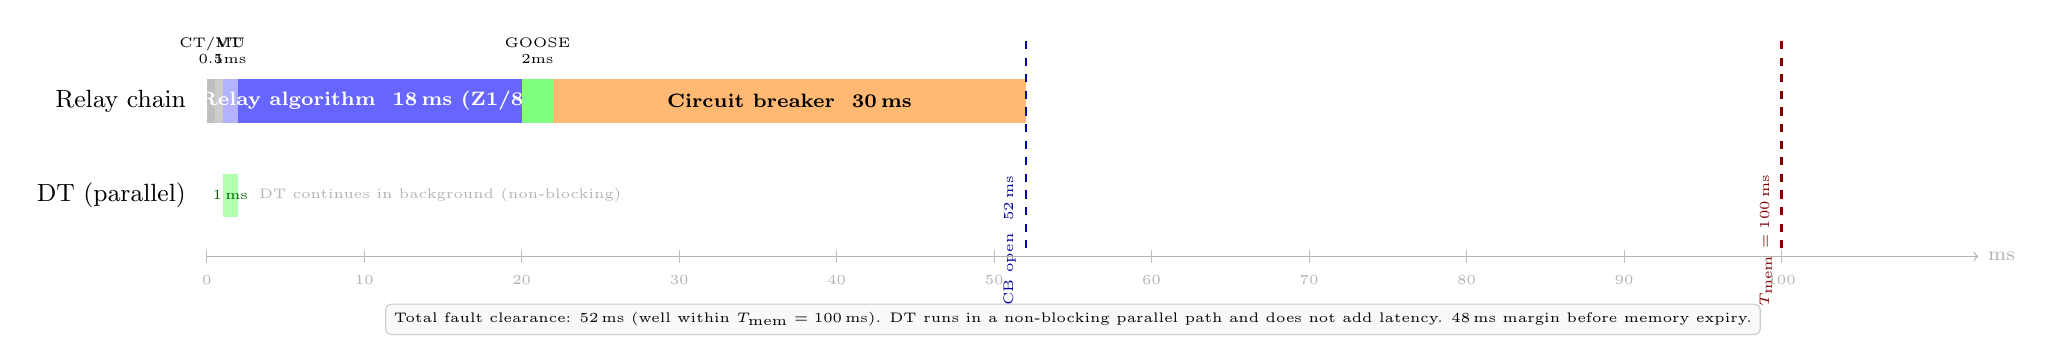
\begin{tikzpicture}[every node/.style={font=\scriptsize}]

\def\bh{0.55}
\def\scale{0.20}  %% 1 ms → 0.20 cm → 1 cm per 5 ms

%% ── Main relay chain (y=0) ────────────────────────────────────────────────────
\node[left=4pt, font=\small] at (0, 0.275) {Relay chain};

%% CT/VT: 0-0.5ms → 0-0.1cm
\fill[gray!50]   (0.0*\scale,0) rectangle (0.5*\scale, \bh);
\node[font=\tiny, above=2pt, align=center] at (0.25*\scale, \bh)
  {CT/VT\\0.5};

%% Sampling: 0.5-1.0ms
\fill[gray!40]   (0.5*\scale, 0) rectangle (1.0*\scale, \bh);

%% MU→relay: 1.0-2.0ms
\fill[blue!30]   (1.0*\scale, 0) rectangle (2.0*\scale, \bh);
\node[font=\tiny, above=2pt, align=center] at (1.5*\scale, \bh)
  {MU\\1ms};

%% Relay algorithm: 2.0-20.0ms (18ms)
\fill[blue!60]   (2.0*\scale, 0) rectangle (20.0*\scale, \bh);
\node[white, font=\scriptsize\bfseries] at (11.0*\scale, 0.275)
  {Relay algorithm \ 18\,ms (Z1/87L)};

%% GOOSE: 20-22ms
\fill[green!50]  (20.0*\scale, 0) rectangle (22.0*\scale, \bh);
\node[font=\tiny, above=2pt, align=center] at (21.0*\scale, \bh)
  {GOOSE\\2ms};

%% CB: 22-52ms
\fill[orange!55] (22.0*\scale, 0) rectangle (52.0*\scale, \bh);
\node[font=\scriptsize\bfseries] at (37.0*\scale, 0.275)
  {Circuit breaker \ 30\,ms};

%% ── DT parallel path (y = -1.2) ──────────────────────────────────────────────
\node[left=4pt, font=\small] at (0, -0.925) {DT (parallel)};

\fill[green!30]  (1.0*\scale, -1.2) rectangle (2.0*\scale, -1.2+\bh);
\node[green!40!black, font=\tiny] at (1.5*\scale, -0.925)
  {1\,ms};
\node[gray!60, font=\tiny, right=4pt] at (2.0*\scale, -0.925)
  {DT continues in background (non-blocking)};

%% ── T_mem limit ────────────────────────────────────────────────────────────────
\draw[red!50!black, thick, dashed]
  (100.0*\scale, -1.60) -- (100.0*\scale, \bh+0.50);
\node[red!50!black, font=\tiny, rotate=90, anchor=south]
  at (100.0*\scale, -1.50)
  {$T_\mathrm{mem}=100$\,ms};

%% Total marker
\draw[blue!70!black, thick, dashed]
  (52.0*\scale, -1.60) -- (52.0*\scale, \bh+0.50);
\node[blue!60!black, font=\tiny, rotate=90, anchor=south]
  at (52.0*\scale, -1.50)
  {CB open \ 52\,ms};

%% ── Axis ────────────────────────────────────────────────────────────────────
\draw[gray!60, ->] (0, -1.70) -- (22.5, -1.70) node[right] {ms};
\foreach \t in {0,10,20,30,40,50,60,70,80,90,100}{
  \draw[gray!50, thin] (\t*\scale, -1.78) -- (\t*\scale, -1.62);
  \node[gray!60, below=1pt, font=\tiny] at (\t*\scale, -1.78) {\t};
}

%% ── Caption ──────────────────────────────────────────────────────────────────
\node[draw=gray!40, fill=gray!5, rounded corners=2pt,
      font=\tiny, inner sep=3pt, align=center]
  at (11.0, -2.50)
  {Total fault clearance: 52\,ms (well within $T_\mathrm{mem}=100$\,ms).
   DT runs in a non-blocking parallel path and does not add latency.
   48\,ms margin before memory expiry.};

\end{tikzpicture}
